\documentclass{report}
\usepackage[utf8]{inputenc}
\usepackage{graphicx}
\DeclareGraphicsExtensions{.pdf,.png,.jpg,.gif}
\usepackage[left=2cm,right=2cm,
    top=2cm,bottom=2cm,bindingoffset=0cm]{geometry}
\usepackage[russian]{babel}
\usepackage{pgfplots}
\pgfplotsset{compat=1.9}
\begin{document}
\renewcommand{\partname}{Билет}
\part{Механическое движение. 
Система отсчета. 
Траектория. Путь. 
Вектор перемещения и его проекции. 
Координатный и векторный способы описания движения. 
Закон движения. 
Скорость. 
Средняя скорость. 
Равномерное прямолинейное движение}

{\bf Механическое движение} ---
изменение пространственного положения тела относительно других тел с течением времени. 

{\bf Траектория} ---
линия, по которой двигалось тело.

{\bf Путь} ---
длина участка траектории, пройденного материальной точкой за данный промежуток времени.

{\bf Перемещение} ---
вектор, проведенный из начального положения материальной точки в конечное. 

{\bf система координат} ---
набор осей, по которым исслудуется движение.

{\bf Материальная точка} ---
тело, обладающее массой, размерами которого можно в данной задаче пренебречь.

{\bf Система отсчета} ---
совокупность тела отсчета, связанной с ним системы координат и часов.

{\bf Средняя скорость} ---
скалярная величина, равная отношению пройденного пути к промежутку времени, 
в течение которого этот путь пройден. 
$$
v_{cp}=\frac{l}{t}
$$

{\bf Скорость} ---
векторная физическая величина, равная пределу отношения перемещения тела к промежутку 
времени, в течение которого это перемещение произошло.
Физический смысл: быстрота изменения координаты.
$$
\vec{v}=\lim_{\Delta t\rightarrow 0}\frac{\Delta \vec{r}}{\Delta \vec{t}}
$$

{\bf Уравнение движения} ---
зависимость координаты от времени
$$
x=x_0+S
$$
уравнение движения позволяет определяить положение тела в любой момент времени.

{\bf Равномерное прямолинейное движение} ---
равномерным называется движение, при котором тело за любые равные промежутки времени 
проходит одинаковые пути.
$$
x=x_0+vt
$$

{\bf Физический смысл скорости движения} ---
быстрота изменения координат.



\part{Неравномерное движение. 
Мгновенная скорость. 
Ускорение. 
Равноускоренное движение. 
Закон равноускоренного движения. 
Графики координаты и скорости при равноускоренном движении. 
Криволинейное движение. 
Скорость и ускорение при криволинейном движении.}

{\bf Неравномерное движение} ---
тело за любые равые промежутки времени проходит неравное количество пути.

{\bf Мгновенная скорость} ---
скорость тела в данный момент времени.

{\bf Ускорение} ---
физическая фелечина, равная отношению изменения скорости к промежутку времени, за 
которое это изменение произошло.
Физический смысл: быстрота изменения скорости.
$$
a=\frac{\Delta v}{\Delta t}
$$

{\bf Равноускоренное движение} ---
движение, при котором скорость изменяется на одинаковую величину за равные отрезки времени.
$$
\vec{v}= \vec{v_0}+\vec{a} \Delta t
$$



\part{Центростремительное и тангенциальное ускорения.}

{\bf Центростремительное ускорение} ---
ускорение, характеризующее быстроту изменения направления линейной скорости при 
движении точки по окружности. Любое криволинейное движение, можно разбить на 
дуги, по которым движется тело.
Пермендекилярно вектору скорости.
$$
a=\frac{v^2}{R}
$$

{\bf Тангенциальное ускорение} ---
ускорение тела, сонаправленное вектору движения. Изменение линейной скорости тела.
$$
a=\frac{\Delta v}{\Delta t}
$$




\part{Движение тела, брошенного под углом к горизонту. 
Закон движения. 
Траектория движения и её уравнение. 
Дальность полета и максимальная высота подъема.
Центростремительное и тангенциальное ускорение. 
Движение по окружности. 
Угловая скорость и угловое ускорение. 
Связь между угловыми и линейными характеристиками движения. 
Период и частота.}

{\bf Движение тела, брошенного под углом к горизонту} ---
тело брошенное под углом $\alpha$ и скоростью $v$ движется в пространстве под 
действием силы тяжести.
Горизонтальная составляющая сткорости $v\cos{\alpha}$, вертикальная состовляющая
$v\sin{\alpha}-gt$

{\bf Траектория} ---
линия, по которой двигалось тело.
$$
\{x,y,z\}=\{x_0+S_x, y_0+S_y, y_0+S_y\}
$$

{\bf Максимальная дальность полета} ---
$$
L=\frac{v^2_0\sin{2\alpha}}{g}
$$

{\bf Максимальная высота полета} ---
$$
H=\frac{v^2_0sin^2{\alpha}}{2g}
$$

{\bf Движение по окружности} ---
криволинейное движение, траекторией которого является окружность.

{\bf Период} ---
время одного полного оборота.
$$
T=\frac{t}{N}
$$

{\bf Частота} ---
количество оборотов за 1 секунду.

$$
\mathcal{V} = \frac{N}{t}
$$

{\bf Угловая скорость} ---
отношение угла поворота ко времени поворота.
$$
\omega =\frac{\lambda}{\Delta t}
$$

{\bf Угловая скорость при равномерном движении} ---
количество оборотов за $2\pi$ секунд.
$$
\omega =\frac{2\pi}{T}=2\pi \mathcal{V}
$$

{\bf Скорость движения по окружности} ---
$$
v=\frac{2\pi R}{T}=2\pi R \mathcal{V} = \omega R
$$



\part{Относительность механического движения. 
Формула сложения скоростей. 
Закон инерции Галилея. 
Первый закон Ньютона. 
Инерциальные системы отсчета. }

{\bf Закон Галилея. Относительное движение тел} ---
скорость тела относительно неподвижной системы отсчета равняется векторной 
сумме скорости тела относительно подвижной системы отсчета и скорости 
подвижной системы отсчета относительно неподвижной.
$$
v=v_1+v_2
$$

{\bf Иннерция} ---
явление сохранения телом скорости по направлению и значению.

{\bf Инертность} ---
Свойство тела сохранять свою скорость по напрвлению и значению.

{\bf Масса} ---
мера инертности.

{\bf Инерциальная система отсчета} ---
система отсчета, тело отсчета которого движется равномено и прямолинейно или покоится.

{\bf Первый закон Ньютона} ---
существую такие системы отсчета, относительно которых тела движутся равномерно и прямолинейно или 
покоятся, если на них не действует сила или действие сил компенсируется.



\part{ Масса. 
Сила. 
Второй закон Ньютона. 
Сложение сил. 
Измерение сил. 
Взаимодействие тел. 
Третий закон Ньютона. 
Принцип относительности Галилея.}

{\bf Масса} ---
мера инертности.

{\bf сила} ---
мера взаимодействия.

{\bf Второй закон Ньютона} ---
ускорение тела прямо пропорционально равнодействующей всех сил, действующих на тело, и обратно
пропорионально массе этого тела
$$
\vec{a}=\frac{\vec{F}}{m}
$$

{\bf Третий закон Ньютона} ---
при взаимодействии возникает две силы, равные по занчению друг-другу по велечине и противоположные
по направлению, приложенные к разным телам.

{\bf Равнодействующая всех сил} ---
векторная сумма всех сил, действующих на тело.



\part{Сила упругости. 
Упругие и неупругие деформации. 
Закон Гука. 
Модуль Юнга. 
Движение под действием силы упругости. 
Силы трения. 
Сухое трение: трение покоя и скольжения. 
Коэффициент трения. 
Вязкое трение. 
Движение под действием силы трения. 
Движение и трение покоя. 
Тормозной путь. 
Время торможения.}

{\bf Дефформирование} ---
изменение формы или объема тела. Дефформации бывают:
\begin{enumerate}
  \item Упругие исчезают после перкращения действия деформирующей силы.
  \item Пластические (не упругие) - чистично или полностью сохраняется после прекращения действия 
  деформирующей силы.
\end{enumerate}

{\bf Сила упругости} ---
сила, возникающая в теле в результате его деформации и стремящаяся вернуть тело в исходное положение.

{\bf Закон Гука} ---
деформация, возникающая в упругом теле, пропорциональна приложенной к этому телу силе.
$$
F=k\Delta l
$$

{\bf Модуль Юнга} ---
механическая характеристика тела. $[E]$
$$
k=\frac{ES}{L}
$$

{\bf Относительное удлинение} ---
$$
\mathcal{E}=\frac{\Delta l}{L}
$$

{\bf Нормальное напряжение в поперечном сечении} ---
$$
\sigma=\frac{F}{S}
$$

{\bf Закон гукадля относиельных велечин} ---
$$
\sigma =E\mathcal{E}
$$

{\bf Закон Гука в относительной форме} ---
$$
\Delta l=\frac{FL}{ES}
$$

{\bf Сила трения} ---
сила, возникающая между поверхностями соприкосающихся тел.
Сила сухого трения прямо пропорциональна силе, прижимающей 
поверхности друг к другу и направлена в сторону, противоположную возможному движению
$$
F=\mu N
$$

{\bf Сухое трение} ---
трение, при котором между поверхностями отсутствует смазка. 

{\bf Трение покоя} ---
трение покоящегося тела, прямо пропорционально силе, пытающейся вывести тело из состояния покоя.

{\bf Вязкое трение} ---
трение среды (воздуха, жидкости).



\part{Гравитационная сила. 
Закон всемирного тяготения. 
Сила тяжести. 
Зависимость силы тяжести от высоты. 
Инертная и гравитационная массы. 
Вес тела. 
Вес тела, движущегося с ускорением. 
Невесомость. 
Перегрузки. 
Движение под действием гравитационной силы. 
Движение планет и искусственных спутников. 
Первая космическая скорость. }

{\bf Сила всемирного тяготения} ---
прямо пропорционально массе каждого из взаимодействующих тел и обратно пропорцианально квадрату
расстояния между их центрами. Сила всемирного тяготения приложена к центрам масс взаимодействующих
тел и направлена по линии, соединящий их центры.
$$
F=G\frac{m_1m_2}{R^2}
$$ 

{\bf Зависимость силы тяжести от высоты} ---
квадратичная.
$$
F=G\frac{m_1m_2}{(R+h)^2}
$$

{\bf Гравитационное поле} ---
это особый вид материи, возникающий в пространстве, содержащей массу. Свойства:
\begin{enumerate}
  \item Материально, т. е. существует.
  \item Убывает с расстоянием.
  \item Непрерывно.
  \item Проявляет себя только в гравитационном воздействии.
\end{enumerate}

{\bf Инертная и гравитационная массы} ---
% TODO

{\bf Вес тела} ---
это сила, с которой тело давит на опору или растягивает подвес.
$$
P=mg
$$

{\bf Вес тела, движущегося с ускорением} ---
при двидении вверх и вниз.
$$
  \begin{array}{ccccc}
    P=mg + ma &&&& P=mg-ma 
  \end{array}
$$

{\bf Невесомость} ---
состояние отсутствия взаимодействия с опорой.

{\bf Первая космическая скорость} ---
минимальная скорость, необходимая скорость, чтобы оставаться на постоянной орбите.
$$
  \begin{array}{ccccc}
    m\frac{v^2}{R}=G\frac{Mm}{R^2} &&&& v=\sqrt{G\frac{M}{R}}
  \end{array}
$$



\part{Импульс материальной точки. 
Импульс силы. 
Импульс системы материальных точек. 
Закон сохранения импульса. 
Условия выполнения закона сохранения импульса. 
Реактивное движение.}

{\bf Импульс тела} ---
векторная физическая велечина, характеризующая способность тела к возможному взаимодействию.
$$
\vec{p}=m\vec{v}
$$

{\bf Импульс силы} ---
векторная физическая велечина, характеризующаявоздействие одного тела на другое.
$$
\vec{I}=\vec{F}\Delta t
$$

{\bf Импульс системы материальных точек} ---
если система находится в покое, то сумма всех испульсов внутренних тел равняется $0$.

{\bf II Закон Ньютона в импульсной форме} ---
$$
F\Delta t=m\vec{v_2}-m\vec{v_1}
$$

{\bf Закон сохранения импульса} ---
Векторная сумма импульсов взаимодействующих тел не изменяется при любых взаимодействях в
замкнутой системе.
$$
m_1\overrightarrow{v_{01}}-m_2\overrightarrow{v_{02}}=
m_1\overrightarrow{v_1}+m_2\overrightarrow{v_2}
$$

{\bf Замкнутая система} ---
система, в которой тела взаимодействуют только между собой.

{\bf Выполнение ЗСИ} ---
закон сохранения импульса выполняется в векторном виде для систем взаимодействующих
сил, для которых равнодействующая внешних сил не изменила своего значения.



\part{Механическая работа. 
Кинетическая энергия материальной точки. 
Теорема о кинетической энергии. 
Зависимость механической работы от траектории движения. 
Мощность.}

{\bf Механическая работа} ---
сила совершает механическую работу, если под действием этой силы тело перемещается.
Числено механическую работу находим как площадь финуры под графиком зависимости силы от 
пройденного пути.
$$
A=FS\cos{\alpha}
$$

{\bf Работа} ---
мера измерения энергии.

{\bf Кинетическая энергия} ---
энергия движения. Это физическая величина, характеризующая движущееся тело.
$$
W_\textrm{к}=\frac{mv^2}{2}
$$

{\bf Мощность} ---
физическая велечина, равная отношению работы к промежутку времени, за которое она совершена.
$$
P=\frac{A}{t}
$$



\part{Полная механическая энергия. 
Закон сохранения полной механической энергии. 
Условия выполнения закона сохранения энергии. 
Изменение механической энергии. 
Работа силы трения и изменение механической энергии.}

{\bf Полная механическая энергия} ---
сумма потенциальной и кинетической энергии.
$$
W_\textrm{полн.мех.эн.}=W_\textrm{к}+W_\textrm{п}
$$

{\bf Закон сохранения полной механической энергии} ---
Полная механическая энергия замкнутой системы физических тел, 
между которыми действуют консервативные силы, является величиной постоянной.

{\bf Изменение механической энергии} ---
работа внешних сил в замкнутой системе равна изменению полной механической энергии.
$$
A_\textrm{дисс}+A_\textrm{нестац}+A_\textrm{вн}=\Delta W_\textrm{полн.мех.эн.}
$$

{\bf Нестационарные силы} ---
силы, велечина которыхзависит от длительности воздействия.

\part{Консервативные и неконсервативные силы. 
Работа консервативной силы. 
Потенциальная энергия. 
Потенциальная энергия силы упругости и силы тяжести.}

{\bf Консервативые силы} ---
силы, работа которых не зависит от вида траектории и определяется только 
начальным и конечным положением этой точки.

Примеры: сила тяжести, сила упругости, гравитационная сила.

{\bf Потенциальная энергия} ---
энергия взаимодействия.

{\bf Потенциальная энергия упругости} ---
$$
W_\textrm{п}=\frac{kx^2}{2}
$$

{\bf Потециальная энергия тяжести} ---
$$
W_\textrm{п}=mgh
$$



\part{Особенности жидкостей. 
Давление. 
Закон Паскаля.
Гидравлический пресс.
Гидростатическое давление. 
Атмосферное давление. 
Опыт Торричелли.}

{\bf Особенности жидкостей} ---
\begin{enumerate}
  \item В расположении молекул жидкости существует ближний порядок и отсутствует дальний.
  \item Молекулы жидкости движутся по всему объему "перескоками" в свободные от молекул
    простраства ("дырки"). Тякучесть жидкости обусловлена перескоками молекул.
  \item Внутренняя энергия жидкости --- сумма кинетической энергии движения молекул и 
    потенциальной энергии их взаимодействия.
\end{enumerate}

{\bf Давление} ---
скалярная физическая величина, равная силе, действующей на единицу площади поверхности. 
$$
p=\frac{F}{S}
$$

{\bf Закон Паскаля} ---
давление, которое оказывается на жидкость или газ, передается в каждую точку 
жидкости или газа без изменений

{\bf Гидравлический пресс} ---
эта машина для оказания статического воздействия - 
сжатия, обработки давлением, зажимания, кинематическим звеном которой является жидкость.
$$
\frac{F_1}{S_1}=\frac{F_2}{S_2}
$$

{\bf Гидрастатическое давление} ---
давление столба воды над условным уровнем. 
$$
p=\rho gh
$$

{\bf Атмосферное давление} ---
давление столба воздуха на земную поверхность.

{\bf Опыт Торричелли} ---
опыт для измерения атмосферного давления. Торричелли наполнил ртутью 
стеклянную трубку длиной около 1 м, запаянную с одного конца. Плотно закрыв 
открытый конец трубки, он её перевернул, опустил в чашку с ртутью и под ртутью 
открыл конец трубки. Часть ртути вылилась в чашку, а часть её осталась в трубке. 
Высота столба ртути, оставшейся в трубке, оказалась равной примерно 760 мм. Над 
ртутью в трубке образовалось безвоздушное пространство.
Измерив высоту столба ртути, можно рассчитать давление, которое производит ртуть. 
Оно и будет равно атмосферному давлению.



\part{Движение жидкости. 
Движение жидкости по трубам. 
Уравнение неразрывности. 
Уравнение Бернулли. 
Следствия из уравнения Бернулли.}

{\bf Уравнение неразрывности жидкости} ---
$$
S_1v_1=S_2v_2
$$

{\bf Уравнение Бернулли} ---
$$
p_1+\rho gh_1+\frac{\rho v_1^2}{2}=p_2+\rho gh_2+\frac{\rho v_2^2}{2}
$$



\part{Твердое тело. 
Структура и свойства твердых тел.}

{\bf Твердое тело} ---
агрегатное состояние вещества, характеризующееся стабильностью формы и характером 
теплового движения атомов, к-рые совершают малые колебания около положений равновесия

Твердые вещества могут быть в кристалическом и аморфном состоянии.

В расположении атомов твердого тела существует ближний и дальний порядок.

Потенциальная энергия взаимодействия вещества имеет минимально возможное значение.

{\bf Кристаллы} ---
это твердые вещества, атомы которого занимают определенное упорядоченное положение в пространстве.

Кристаллические вещества могут состоять из монокристалов и полекристалов.

{\bf Монокристал} ---
одиночный кристал.

Физические свойстава:
\begin{enumerate}
  \item Правильная геометрическая форма.
  \item Постоянная темпера плавления.
  \item Анизонтропия --- неодинаковость свойств среды. 
\end{enumerate}

{\bf Поликристал} ---
это совокупность сросшихся между собой монокристалов.

Физические свойстава:
\begin{enumerate}
  \item Правильная форма.
  \item Постоянная температура плавления.
  \item Изотропия --- постоянство свойств среды.
\end{enumerate}

{\bf Аморфные} ---
нет дальнего порядка.

Физические свойстава:
\begin{enumerate}
  \item Обладает свойством тякучести.
  \item Не имеют постоянной темепературы плавления.
\end{enumerate}



\part{Абсолютно твердое тело. 
Момент силы относительно оси вращения. 
Сложение моментов сил. 
Правило моментов. 
Равновесие тел. 
Виды положений равновесия.}

{\bf Абсолютно твердое тело} ---
модельное понятие классической механики, обозначающее совокупность материальных 
точек, расстояния между которыми сохраняются в процессе любых движений, совершаемых этим телом.

{\bf Момент силы} ---
произведение модуля силы $\vec{F}$ на ее плечо $d$, где плечо $d$ — 
расстояние от точки $O$ до линии действия силы $\vec{F}$. 
$$
M=Fd
$$

{\bf Сложение моментов сил} ---
Если сила вращает тело по часовой стрелке, то момент этой силы надо брать со знаком $-$.
Иначе если сила вращает тело по часовой стрелке, то момент этой силы надо брать со знаком $+$.

{\bf Правило моментов} ---
если тело находится в равновесии (не вращается), то сумма моментов сил, врощающих тело по часовой
стрелке, равна сумме моментов сил, вращающих тело против часовой стрелке.

{\bf Равновесие тел}
\begin{enumerate}
  \item Тело двидется равномерно или покоится. I закон Ньютона:
  $$
  \vec{F_1}+\vec{F_2}+\dots+\vec{F_n}=0
  $$
  \item Тело не вращается. Правило моментов:
  $$
  M_1+M_2+\dots+M_n=0
  $$
\end{enumerate}

{\bf Следствие из уравнения Бернулли} ---
% TODO



\part{Молекулярное строение вещества. 
Основные положения молекулярно-кинетической теории и их опытное обоснование. 
Моль вещества. 
Постоянная Авогадро.
Размеры и массы молекул. 
Скорости молекул. 
Опыт Штерна.  }

{\bf Основные положения маллекулярно-кинетической теории}:
\begin{enumerate}
  \item Все вещества состоят из молекул. 
  Опытное обоснование: если тереть вещество, то оно постепенно стирается.
  \item Все молекулы вещества находятся в непрекращающимся хаотичном движении.
  Опытное обоснование: Броуновское движение, опыт Штерна.
  \item Молекулы вещества взаимодействуют между собой силами взаимодействия и отталкивания.
\end{enumerate}

{\bf Броуновское движение} ---
движение взвешенных частиц в жидкости или газе. Примеры: хаотичное движение малых частиц в воде,
пыль в комнате.

{\bf Моль вещества} ---
это количество вещества, в котором содержится столько же частиц, сколько атомов 
содержится в $12$ граммах углерода с атомной единицей массы $12$. 

{\bf Молярная масса} ---
масса одного моля вещества
$$
\mathcal{M}=m_0N_A
$$

{\bf Постоянная Авогадро} ---
это число атомов (молекул, или других структурных элементов вещества), содержащихся в 1 моле.
$$
N_a=6\cdot10^{23}\frac{1}{\textrm{моль}}
$$

{\bf Количество вещества}:
$$
\mathcal{V}=\frac{m}{\mathcal{M}}=\frac{N}{N_A}
$$

{\bf Опыт Штерна} ---
% TODO



\part{Давление газа. 
Идеальный газ. 
Основное уравнение молекулярно-кинетической теории.
Изопроцессы. 
Графики изопроцессов.}

{\bf Давление газа} ---
%TODO

{\bf Идеальный газ} ---
физическая модель реального газа. В идеальном газе принебрегается:
\begin{enumerate}
  \item Взаимодействием молекул силами притяжения и отталкивания.
  \item Размерами молекул.
\end{enumerate}

{\bf Основное уравнение молекулярно-кинематической теории}:
$$
p=\frac{2}{3}nE_{\textrm{к}0}
$$

{\bf Изотермический процесс. Закон Бойля-Мариота} ---
для данной массе газа, при неизменной температуре произведние давления на 
объем является велечиной постоянной.
$$
T_1=T_2=\textrm{const} \qquad 
p_1V_1=p_2V_2 \qquad 
p(V)=\frac{1}{V}
$$

{\bf Изобарный процесс. Закон Гей-Люсака} ---
для данной массы газа при неизменном давлении отношение объема к абсолютной 
температуре остается неизменной.
$$
p_1=p_2=\textrm{const} \qquad 
\frac{V_1}{T_1}=\frac{V_2}{T_2} \qquad
V(T) = T
$$

{\bf Изокорный процесс. Закон Шарля} ---
для данной массе газа и при неизменном объеме отнощение давления к абсолютной темепературе
остается постоянным.
$$
V_1=V_2=\textrm{const} \qquad 
\frac{P_1}{T_1}=\frac{P_2}{T_2} \qquad
P(T) = T
$$



\part{Температура, ее физический смысл. 
Абсолютная температура. 
Абсолютный ноль температуры. 
Шкала температур Цельсия.}

{\bf Температура} ---
физическая велечина, характеризующая степень нагретости тела. Это параметр одинаков для всех 
веществ, находящихся в тепловом равновесии. Мера средней кинетической энергии молекулы.
$$
E_{ko}=\frac{3}{2}kT \qquad k=1.38\cdot 10^{-23}\frac{\textrm{Дж}}{\textrm{k}^\circ}
$$

{\bf Абсолютный ноль} ---
минимальная температура, при которой скорость молекулы рана нулю.
$$
t_0=-273^\circ
$$

{\bf Абсолютная температура} ---
начинает отсчет с абсолютного нуля.
$$
T=t-273^\circ
$$



\part{Внутренняя энергия. 
Параметры состояния.}

{\bf Внутренняя энергия идеального газа}:
% TODO
$$
U=\frac{m_0v^2}{2}N=\frac{i}{2}\frac{m}{\mathcal{M}}RT
$$

$i$ --- число степеней свободы молекул.

{\bf Параметры состояния} ---
% TODO



\part{Количество теплоты. 
Работа газа. 
Первое начало термодинамики.
Идеальный тепловой двигатель. 
КПД идеального двигателя. 
Тепловые двигатели. 
КПД тепловых двигателей. 
Второе начало термодинамики. 
Обратимые и необратимые процессы. 
Обратимость термодинамических процессов.}

{\bf Количество теплоты} ---
мера изменения внутренней энергии тела при теплообмене.

{\bf Первое начало термодинамики} ---
Изменение $\Delta U$ внутренней энергии неизолированной термодинамической системы равно разности 
между количеством теплоты $Q$, переданной системе, и работой $A$, совершенной системой над 
внешними телами.
$$
Q=\Delta U + A
$$

{\bf Идеальный тепловой двигатель} ---

\begin{figure}[bh]
  \noindent\centering{
    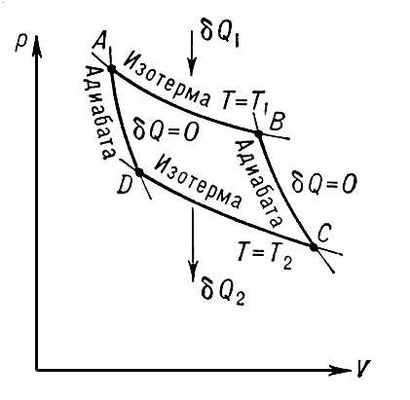
\includegraphics[width=30mm]{0001.png}
  }
  \caption{График двигателя карно}
\end{figure}

{\bf КПД идеального теплового двигателя} ---
двигатель карно из 2х адиабат и 2х изотерм.
$$
\eta = \frac{T_\textrm{н.}-T_\textrm{х.}}{t_\textrm{н.}}
$$

{\bf Тепловые двигатели} ---
это устройства, в котором внутренняя энергия газа превращается в механическую работу.

{\bf КПД тепловых двигателей}:
$$
\eta = \frac{A}{Q_\textrm{н}}=\frac{Q_\textrm{н}-\left|Q_\textrm{х}\right|}{Q_\textrm{н}}
$$



\part{Кристаллическая и аморфная структура вещества. 
Удельная теплота плавления.}

{\bf Твердое тело} ---
агрегатное состояние вещества, характеризующееся стабильностью формы и характером 
теплового движения атомов, к-рые совершают малые колебания около положений равновесия

Твердые вещества могут быть в кристалическом и аморфном состоянии.

В расположении атомов твердого тела существует ближний и дальний порядок.

Потенциальная энергия взаимодействия вещества имеет минимально возможное значение.

{\bf Кристаллы} ---
это твердые вещества, атомы которого занимают определенное упорядоченное положение в пространстве.

Кристаллические вещества могут состоять из монокристалов и полекристалов.

{\bf Монокристал} ---
одиночный кристал.

Физические свойстава:
\begin{enumerate}
  \item Правильная геометрическая форма.
  \item Постоянная темпера плавления.
  \item Анизонтропия --- неодинаковость свойств среды. 
\end{enumerate}

{\bf Поликристал} ---
это совокупность сросшихся между собой монокристалов.

Физические свойстава:
\begin{enumerate}
  \item Правильная форма.
  \item Постоянная температура плавления.
  \item Изотропия --- постоянство свойств среды.
\end{enumerate}

{\bf Аморфные} ---
нет дальнего порядка.

Физические свойстава:
\begin{enumerate}
  \item Обладает свойством тякучести.
  \item Не имеют постоянной темепературы плавления.
\end{enumerate}



\part{Поверхностные явления.
Энергия поверхностного слоя.
Сила поверхностного натяжения.
Давление под искривленной поверхностью жидкости.
Явление смачивания и несмачивания.
Капиллярные явления.}

{\bf Поверхностные явления} ---
% TODO

{\bf Энергия поверхностного слоя}:
$$
W_\textrm{п.сл.}=\sigma S
$$
$$
\sigma \textrm{--- коэффициент поверхностного натяжения.}
$$

{\bf Сила поверхностного натяжения}:
$$
F_\textrm{пов.нат.}=\sigma l
$$
$$
l \textrm{--- длинна контура жидкости.}
$$

{\bf Лапласово давление} ---
дополнительное давление, которое создает искривленная поверхность жидкости, стремящаяся 
выпрямиться под действием молекулярных сил. Это давление при смачивании (вогнутый мениск) 
направлено от жидкости, а при несмачивании (выпуклый мениск) — внутрь.
$$
p=\frac{2\sigma}{R}
$$

{\bf Миниск} ---
искривленная поверхность жидкости на границе с твердым телом.
Выпуклый миниск - не смачивает твердое тело.
Вогнутый миниск - смачивает.

{\bf Капилярные явления} ---
$$
h=\frac{2\sigma}{\rho g r}
$$


\part{Границы применимости законов идеального газа. 
Насыщенный и ненасыщенный пар. 
Зависимость давления и плотности насыщенного пара от температуры. 
Зависимость температуры кипения от давления. 
Влажность.
Измерение относительной влажности.}

{\bf Границы применения законов идеального газа} ---
% TODO

{\bf Испарение} ---
парообразование с поверхности жидкости.

Скорость испарения зависит от 
\begin{enumerate}
  \item Температуры жидкости
  \item Площади поверхности
  \item Вязкости жидкости
  \item Скорости потока газа над жидкостью
  \item 
\end{enumerate}

{\bf } ---

{\bf } ---

{\bf } ---

{\bf } ---

{\bf } ---

{\bf } ---

{\bf } ---

{\bf } ---

{\bf } ---

{\bf } ---

{\bf } ---

{\bf } ---

{\bf } ---

{\bf } ---

{\bf } ---

{\bf } ---

{\bf } ---

{\bf } ---

{\bf } ---

{\bf } ---

{\bf } ---

{\bf } ---

{\bf } ---

{\bf } ---

{\bf } ---

{\bf } ---

{\bf } ---

{\bf } ---

{\bf } ---

{\bf } ---

{\bf } ---

{\bf } ---

{\bf } ---

{\bf } ---

{\bf } ---

{\bf } ---

{\bf } ---

{\bf } ---

{\bf } ---

{\bf } ---

{\bf } ---

{\bf } ---

{\bf } ---

{\bf } ---

{\bf } ---

{\bf } ---

{\bf } ---

{\bf } ---

{\bf } ---

{\bf } ---

{\bf } ---

{\bf } ---

{\bf } ---

{\bf } ---

{\bf } ---

{\bf } ---

{\bf } ---

{\bf } ---

\end{document}